\documentclass[tikz,border=12pt]{standalone}
\usepackage[T1]{fontenc}
\usepackage{mathpazo}
\usepackage{amsmath,amssymb}
\usetikzlibrary{arrows.meta, positioning, calc}

\definecolor{stblue}{HTML}{7B97AD}
\definecolor{rwgold}{HTML}{B8995E}
\definecolor{sage}{HTML}{7A9A7E}
\definecolor{dkbrown}{HTML}{3D3530}
\definecolor{wmgray}{HTML}{7B7067}
\definecolor{cream}{HTML}{F9F6F0}
\definecolor{border}{HTML}{D4C9B8}
\definecolor{terracotta}{HTML}{C47A6A}
\definecolor{lavender}{HTML}{907EA0}

\begin{document}
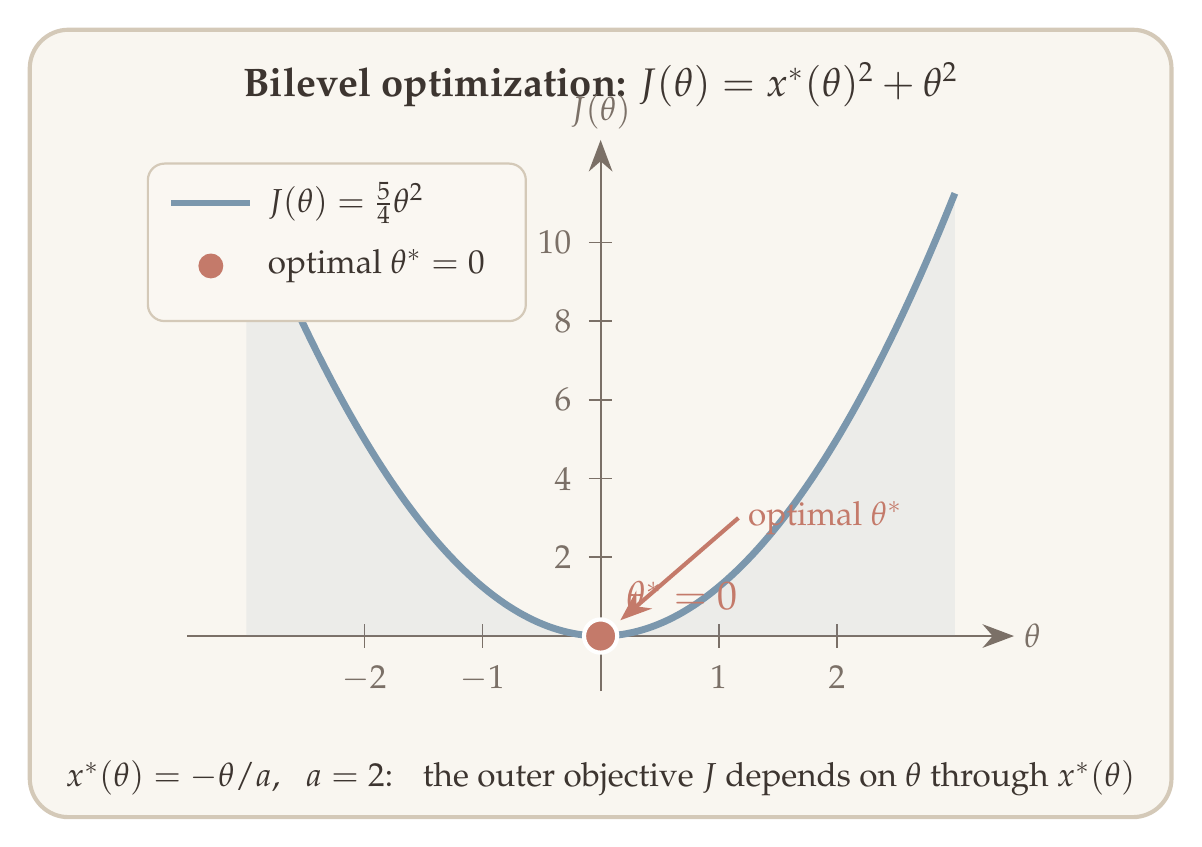
\begin{tikzpicture}[>={Stealth[length=4mm, width=3mm]}]

% Background
\fill[cream, rounded corners=14pt] (-0.5,-0.8) rectangle (14,9.2);
\draw[border, line width=1.5pt, rounded corners=14pt] (-0.5,-0.8) rectangle (14,9.2);

% Title
\node[text=dkbrown, font=\Large\bfseries] at (6.75,8.5)
  {Bilevel optimization: $J(\theta) = x^*(\theta)^2 + \theta^2$};

% Coordinate mapping:
% theta-range: -3 to 3, center at canvas x=6.75
% y-range: -0.5 to 12, anchor at canvas y=1.5
% x-scale: 1.5, y-scale: 0.5

% Axes
\draw[wmgray, line width=0.8pt, ->] (1.5,1.5) -- (12.0,1.5)
  node[right, font=\large, text=wmgray] {$\theta$};
\draw[wmgray, line width=0.8pt, ->] (6.75,0.8) -- (6.75,7.8)
  node[above, font=\large, text=wmgray] {$J(\theta)$};

% theta -> 6.75 + theta*1.5
% y -> 1.5 + y*0.5

% Tick marks theta-axis
\foreach \t/\lab in {-2/-2, -1/-1, 1/1, 2/2} {
  \draw[wmgray, line width=0.6pt] ({6.75+\t*1.5},1.35) -- ({6.75+\t*1.5},1.65);
  \node[text=wmgray, font=\large, below] at ({6.75+\t*1.5},1.25) {$\lab$};
}

% Y-axis ticks
\foreach \v in {2,4,6,8,10} {
  \draw[wmgray, line width=0.6pt] (6.6,{1.5+\v*0.5}) -- (6.9,{1.5+\v*0.5});
  \node[text=wmgray, font=\large, left] at (6.5,{1.5+\v*0.5}) {\pgfmathprintnumber[fixed]{\v}};
}

% J(theta) = x*(theta)^2 + theta^2 = (-theta/2)^2 + theta^2 = theta^2/4 + theta^2 = 5/4 * theta^2
% with a = 2

% Fill under curve
\fill[stblue, opacity=0.1]
  plot[smooth, domain=-3:3, samples=50] ({6.75 + \x*1.5}, {1.5 + 1.25*\x*\x*0.5})
  -- (11.25, 1.5) -- (2.25, 1.5) -- cycle;

% Plot J(theta) = 1.25 * theta^2
\draw[stblue, line width=2.5pt] plot[smooth, domain=-3:3, samples=50]
  ({6.75 + \x*1.5}, {1.5 + 1.25*\x*\x*0.5});

% Optimal point theta* = 0
\fill[terracotta] (6.75,1.5) circle (6pt);
\draw[white, line width=1.5pt] (6.75,1.5) circle (6pt);
\node[text=terracotta, font=\Large\bfseries, above right=4pt] at (6.85,1.6)
  {$\theta^* = 0$};

% Arrow pointing to minimum
\draw[terracotta, line width=1.5pt, ->] (8.5,3.0) -- (7.0,1.7);
\node[text=terracotta, font=\large, right] at (8.5,3.0) {optimal $\theta^*$};

% Legend
\fill[cream!90!white, rounded corners=6pt] (1.0,5.5) rectangle (5.8,7.5);
\draw[border, line width=0.8pt, rounded corners=6pt] (1.0,5.5) rectangle (5.8,7.5);

\draw[stblue, line width=2.5pt] (1.3,7.0) -- (2.3,7.0);
\node[text=dkbrown, font=\large, right] at (2.4,7.0) {$J(\theta) = \tfrac{5}{4}\theta^2$};
\fill[terracotta] (1.8,6.2) circle (4.5pt);
\node[text=dkbrown, font=\large, right] at (2.4,6.2) {optimal $\theta^* = 0$};

% Bottom annotation
\node[text=dkbrown, font=\large] at (6.75,-0.3)
  {$x^*(\theta) = -\theta/a$, \; $a = 2$: \; the outer objective $J$ depends on $\theta$ through $x^*(\theta)$};

\end{tikzpicture}
\end{document}
